\chapter{Sets, Etc.}

\section{Sets}

\begin{enumerate}

\item[B.1{-}1] {Draw Venn diagrams that illustrate the first of the distributive
laws (B.1).}

\begin{framed}
\begin{center}
\def\firstcircle{(0,0) circle (0.5cm)}
\def\secondcircle{(60:0.75cm) circle (0.5cm)}
\def\thirdcircle{(0:0.75cm) circle (0.5cm)}

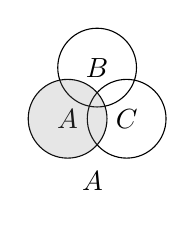
\begin{tikzpicture}
  \draw \firstcircle node (a) {$A$};
  \draw \secondcircle node (b) {$B$};
  \draw \thirdcircle node (c) {$C$};
  \fill[gray, fill opacity=0.2] \firstcircle;
  \node [align=flush center, below=1.2cm] at (b) { $A$ };
\end{tikzpicture}
\begin{tikzpicture}
  \node [align=flush center,text width=0.5cm, minimum height=0.5cm] at (0,0) { $\cap$ };
  \node [align=flush center,text width=0.5cm, minimum height=0.5cm] at (0,1) { $\cap$ };
\end{tikzpicture}
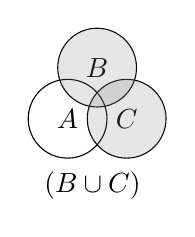
\begin{tikzpicture}
  \draw \firstcircle node (a) {$A$};
  \draw \secondcircle node (b) {$B$};
  \draw \thirdcircle node (c) {$C$};
  \fill[gray, fill opacity=0.2] \secondcircle;
  \fill[gray, fill opacity=0.2] \thirdcircle;
  \node [align=flush center, below=1.2cm] at (b) { $(B \cup C)$ };
\end{tikzpicture}
\begin{tikzpicture}
  \node [align=flush center,text width=0.5cm, minimum height=0.5cm] at (0,0) { $=$ };
  \node [align=flush center,text width=0.5cm, minimum height=0.5cm] at (0,1) { $=$ };
\end{tikzpicture}
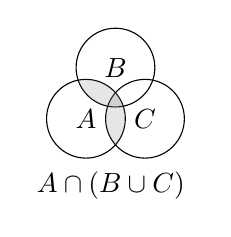
\begin{tikzpicture}
  \draw \firstcircle node (a) {$A$};
  \draw \secondcircle node (b) {$B$};
  \draw \thirdcircle node (c) {$C$};
  \begin{scope}
    \clip \firstcircle;
    \fill[gray, fill opacity=0.2] \secondcircle;
  \end{scope}
  \begin{scope}
    \clip \firstcircle;
    \fill[gray, fill opacity=0.2] \thirdcircle;
  \end{scope}
  \node [align=flush center, below=1.2cm] at (b) { $A \cap (B \cup C)$ };
\end{tikzpicture}
\begin{tikzpicture}
  \node [align=flush center,text width=0.5cm, minimum height=0.5cm] at (0,0) { $=$ };
  \node [align=flush center,text width=0.5cm, minimum height=0.5cm] at (0,1) { $=$ };
\end{tikzpicture}
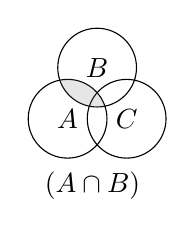
\begin{tikzpicture}
  \draw \firstcircle node (a) {$A$};
  \draw \secondcircle node (b) {$B$};
  \draw \thirdcircle node (c) {$C$};
  \begin{scope}
    \clip \firstcircle;
    \fill[gray, fill opacity=0.2] \secondcircle;
  \end{scope}
  \node [align=flush center, below=1.2cm] at (b) { $(A \cap B)$ };
\end{tikzpicture}
\begin{tikzpicture}
  \node [align=flush center,text width=0.5cm, minimum height=0.5cm] at (0,0) { $\cup$ };
  \node [align=flush center,text width=0.5cm, minimum height=0.5cm] at (0,1) { $\cup$ };
\end{tikzpicture}
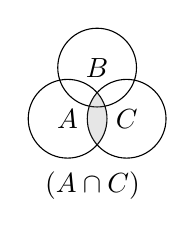
\begin{tikzpicture}
  \draw \firstcircle node (a) {$A$};
  \draw \secondcircle node (b) {$B$};
  \draw \thirdcircle node (c) {$C$};
  \begin{scope}
    \clip \firstcircle;
    \fill[gray, fill opacity=0.2] \thirdcircle;
  \end{scope}
  \node [align=flush center, below=1.2cm] at (b) { $(A \cap C)$ };
\end{tikzpicture}
\end{center}
\end{framed}

\item[B.1{-}2] {Prove the generalization of DeMorgan's laws to any finite
collection of sets:
\[
  \overline{A_1 \cap A_2 \cap \cdots \cap A_n} = \overline{A_1} \cup \overline{A_2} \cup \cdots \cup \overline{A_n},
\]
\[
  \overline{A_1 \cup A_2 \cup \cdots \cup A_n} = \overline{A_1} \cap \overline{A_2} \cap \cdots \cap \overline{A_n}.
\]
}

\begin{framed}
The base case, which occurs when $n = 2$, is given (from the text book). Now,
lets assume it holds for $n$ and show that it also holds for $n + 1$.

For the first DeMongan's law, we have
\begin{equation*}
\begin{aligned}
  \overline{A_1 \cap A_2 \cap \cdots \cap A_n \cap A_{n + 1}}
  &= \overline{(A_1 \cap A_2 \cap \cdots \cap A_n) \cap A_{n + 1}}\\
  &= \overline{(A_1 \cap A_2 \cap \cdots \cap A_n)} \cup \overline{A_{n + 1}}\\
  &= (\overline{A_1} \cup \overline{A_2} \cup \cdots \cup \overline{A_n}) \cup \overline{A_{n + 1}}\\
  &= \overline{A_1} \cup \overline{A_2} \cup \cdots \cup \overline{A_n} \cup \overline{A_{n + 1}}.
\end{aligned}
\end{equation*}

For the second DeMongan's law, we have
\begin{equation*}
\begin{aligned}
  \overline{A_1 \cup A_2 \cup \cdots \cup A_n \cup A_{n + 1}}
  &= \overline{(A_1 \cup A_2 \cup \cdots \cup A_n) \cup A_{n + 1}}\\
  &= \overline{(A_1 \cup A_2 \cup \cdots \cup A_n)} \cap \overline{A_{n + 1}}\\
  &= (\overline{A_1} \cap \overline{A_2} \cap \cdots \cap \overline{A_n}) \cap \overline{A_{n + 1}}\\
  &= \overline{A_1} \cap \overline{A_2} \cap \cdots \cap \overline{A_n} \cap \overline{A_{n + 1}}.
\end{aligned}
\end{equation*}
\end{framed}

\item[B.1{-}3]{($\star$) Prove the generalization of equation (B.3), which is
called the \textbf{\emph{principle of inclusion and exclusion}}:
\begin{equation*}
\begin{aligned}
  | A_1 &\cup A_2 \cup \cdots \cup A_n | =\\
        &|A_1| + |A_2| + \cdots + |A_n|\\
        &- |A_1 \cap A_2| - |A_1 \cap A_3| - \cdots && \text{(all pairs)}\\
        &+ |A_1 \cap A_2 \cap A_3| + \cdots && \text{(all triples)}\\
        &\qquad\qquad\qquad\vdots\\
        &+ (-1)^{n - 1} |A_1 \cap A_2 \cap \cdots \cap A_n|.
\end{aligned}
\end{equation*}
}

\begin{framed}
Skipped.
\end{framed}

\item[B.1{-}4]{Show that the set of odd natural numbers is countable.}

\begin{framed}
Let $\mathbb{O}$ denote the set of odd natural numbers.

The function $f(n) = 2n + 1$ is a 1-1 correspondence from $\mathbb{N}$ to
$\mathbb{O}$.  Thus, $\mathbb{O}$ is countable.
\end{framed}

\newpage

\item[B.1{-}5]{Show that for any finite set $S$, the power set $2^S$ has
$2^{|S|}$ elements (that is, there are $2^{|S|}$ distinct subsets of $S$).}

\begin{framed}
For the base case, consider a set with a single element $x$. We have
\[
  2^{\{x\}} = \{\emptyset, \{x\}\},
\]
which shows that the power set of a set with a single element has cardinality
$2^1 = 2$.

Let $C(\cdot)$ denote the cardinality of a power set. Let $S$ be a set of size
$n$. Lets assume that the power set of $S$ has cardinality
$C(S) = 2^{|S|} = 2^n$. Now, let $S'$ be the set $S$ with one additional element
$x$, such that $|S'| = n + 1$. The power set of $S'$ will consist of all sets
in the power set of $S$ plus all those same sets again, with the element $x$
added. Thus, we have
\[
  C(S') = 2 \cdot C(S) = 2 \cdot 2^n = 2^{n + 1}.
\]
\end{framed}

\item[B.1{-}6]{Give an inductive definition for an $n$-tuple by extending the
set-theoretic definition for an ordered pair.}

\begin{framed}
\begin{equation*}
\begin{aligned}
  (a) &= \{a\}\\
  (a, b) &= \{a, \{a, b\}\}\\
  (a, b, c) &= \{a, \{a, b\}, \{a, b, c\}\}\\
  (a_1, a_2, \dots, a_n) &= (a_1, a_2, \dots, a_{n - 1}) \cup \{a_1, a_2, \dots, a_n\}
\end{aligned}
\end{equation*}
\end{framed}

\end{enumerate}

\newpage

\section{Relations}

\begin{enumerate}

\item[B.2{-}1]{Prove that the subset relation ``$\subseteq$'' on all subsets of
$\mathbb{Z}$ is a partial order but not a total order.}

\begin{framed}
Let $\mathbb{S}$ denote all the subsets of $\mathbb{Z}$. Let $A = \{1\}$,
$B = \{2\}$ be two subsets of $\mathbb{Z}$. We have $A \not\subseteq B$ and
$B \not\subseteq A$. Thus, the subset relation ``$\subseteq$'' on
$\mathbb{S} \times \mathbb{S}$ is not a total relation and therefore is not
a total order.

For the relation $\subseteq$ on $\mathbb{S}$ be a partial order, the
following properties needs to hold: (1) reflexivity, (2) antisymmetry,
(3) transitivity. Since $A \subseteq A$, for all $A \in \mathbb{S}$, the
relation ``$\subseteq$'' on $\mathbb{S} \times \mathbb{S}$ is reflexive. To be
antisymmetric, we need to show that if $A \subseteq B$ and $B \subseteq A$, then
$A = B$, for all $A, B \in \mathbb{S}$. Since $A \subseteq B$, for all $a \in A$
we have $a \in B$ and since $B \subseteq A$, for all $b \in B$ we have
$b \in A$.  Thus, $A = B$ and the relation ``$\subseteq$'' on
$\mathbb{S} \times \mathbb{S}$ is antisymmetric. To be transitive, we need to
show that if $A \subseteq B$ and $B \subseteq C$, then $A \subseteq C$, for all
$A, B, C \in \mathbb{S}$. So let $a \in A$.  Since $A \subseteq B$, we have
$a \in B$. Since $a \in B$ and $B \subseteq C$, we have $a \in C$. Thus,
$A \subseteq C$ and the relation ``$\subseteq$'' on
$\mathbb{S} \times \mathbb{S}$ is transitive.
\end{framed}

\item[B.2{-}2]{Show that for any positive integer $n$, the relation ``equivalent
modulo $n$'' is an equivalence relation on the integers. (We say that
$a \equiv b$ (mod $n$) if there exists an integer $q$ such that $a - b = qn$.)
Into what equivalence classes does this relation partition the integers?}

\begin{framed}
To the relation ``equivalent modulo $n$'' be an equivalent relation on
$\mathbb{Z} \times \mathbb{Z}$, the following needs to hold:
\begin{enumerate}
  \item $a \equiv a$ (mod $n$), for all $a, n \in \mathbb{Z}$ (reflexivity)
  \item $a \equiv b$ (mod $n$) implies $b \equiv a$ (mod $n$), for all $a, b, n \in \mathbb{Z}$ (symmetry)
  \item $a \equiv b$ (mod $n$) and $b \equiv c$ (mod $n$) implies $a \equiv c$ (mod $n$), for all $a, b, c, n \in \mathbb{Z}$ (transitivity)
\end{enumerate}

For the reflexivity property, we have that $a - a = qn$ holds directly for $q = 0$.

For the symmetry property, we have that $a - b = p n$ implies $b - a = q n$ holds directly for $q = -p$.

For the transitivity property, we have that $a - b = pn$ and $b - c = qn$ implies $a - c = rn$ holds for $r = p + q$, since
\[
  (a - b) + (b - c) = pn + qn \rightarrow a - c = (p + q) n.
\]

\end{framed}

\item[B.2{-}3]{Give examples of relations that are
\begin{enumerate}
\item[a.] reflexive and symmetric but not transitive,
\item[b.] reflexive and transitive but not symmetric,
\item[c.] symmetric and transitive but not reflexive.
\end{enumerate}
}

\begin{framed}
\begin{enumerate}
\item The relation ``is neighbor of'' is reflexive (one is neighbor of
  himself) and symmetric ($a$ ``is neighbor of'' $b$ imply $b$ ``is neighbor
  of'' $a$), but not transitive ($a$ ``is neighbor of'' $b$ and $b$ ``is
  neighbor of'' $c$ does not imply $a$ ``is neighbor of'' $c$.
\item The relation ``$\le$'' is reflexive ($a \le a$) and transitive ($a \le b$
  and $b \le c$ imply $a \le c$), but not symmetric ($a \le b$ does not imply
  $b \le a$).
\item Consider the relation ``$a + b > \infty$'' on $\mathbb{Z} \times \mathbb{Z}$.
  This relation is empty. However, it is symmetric ($a\;R\;b$ imply $b\;R\;a$)
  and transitive ($a\;R\;b$ and $b\;R\;c$ imply $a\;R\;c$), but not reflexive
  since for no $a \in \mathbb{Z}$ is it the case that $a\;R\;a$.
\end{enumerate}
\end{framed}

\item[B.2{-}4]{Let $S$ be a finite set, and let $R$ be an equivalence relation
on $S \times S$. Show that if in addition $R$ is antisymmetric, then the
equivalence classes of $S$ with respect to $R$ are singletons.}

\begin{framed}
For every $a, b \in S$ such that $a\;R\;b$, by symmetry $b\;R\;a$, and by
antisymmetry $a = a$. Thus, $[a] = \{b \in S : a\;R\;b\} = \{a\}$ for all
$a \in S$, which implies that the equivalence classes are singletons.
\end{framed}

\item[B.2{-}5]{Professor Narcissus claims that if a relation $R$ is symmetric
and transitive, then it is also reflexive. He offers the following proof. By
symmetry, $a\;R\;b$ implies $b\;R\;a$. Transitivity, therefore, implies
$a\;R\;a$. Is the professor correct?}

\begin{framed}
No. This is only true for relations that for every $a$ there is $b$ such that
$a\;R\;b$, by symmetry $b\;R\;a$, and by transitivity $a\;R\;a$. For
instance, an empty relation (like the one from Question B.2-3, item (c)) are
symmetric and transitive, but not reflexive.
\end{framed}

\end{enumerate}

\newpage

\section{Functions}

\begin{enumerate}

\item[B.3{-}1]{Let $A$ and $B$ be finite sets, and let $f : A \rightarrow B$ be
a function. Show that
\begin{enumerate}
\item[a.] if $f$ is injective, then $|A| \le |B|$;
\item[b.] if $f$ is surjective, then $|A| \ge |B|$.
\end{enumerate}
}

\begin{framed}
\begin{enumerate}
  \item Since $f$ is injective, we have that $A = f(A)$. Also, we have
    \begin{equation*}
    \begin{cases}
      |B| = |f(A)|, & f \text{ is surjective},\\
      |B| > |f(A)|, & f \text{ is not surjective}.
    \end{cases}
    \end{equation*}
    Thus, $|B| \ge |f(A)| = |A| \rightarrow |A| \le |B|$.
  \item Since $f$ is surjective, we have $|f(A)| = |B|$. Also, we have
    \begin{equation*}
    \begin{cases}
      |A| = |f(A)|, & f \text{ is injective},\\
      |A| > |f(A)|, & f \text{ is not injective}.
    \end{cases}
    \end{equation*}
    Thus, $|A| \ge |f(A)| = |B| \rightarrow |A| \ge |B|$.
\end{enumerate}
\end{framed}

\item[B.3{-}2]{Is the function $f(x) = x + 1$ bijective when the domain and the
codomain are $\mathbb{N}$? Is it bijective when the domain and the codomain are
$\mathbb{Z}$?}

\begin{framed}
On the set of naturals, $f$ is injective but not surjective, since there is no
$a \in \mathbb{N}$ such that $0 = f(a)$, which makes
$f(\mathbb{N}) \neq \mathbb{N}$.

On the set of integers, $f$ is both injective and surjective, and therefore
bijective.
\end{framed}

\item[B.3{-}3]{Give a natural definition for the inverse of a binary relation
such that if a relation is in fact a bijective function, its relational inverse
is its functional inverse.}

\begin{framed}
Let $R$ be a binary relation on the sets $A$ and $B$, such that
$R \subseteq A \times B$. The general definition of the inverse of $R$ is given
by
\[
  R^{-1} = \{(b, a) \in B \times A : (a, b) \in R\}.
\]

When $R$ is a bijective function, we have: (1) for all $b \in B$, there
is at most one $a \in A$ such that $a\;R\;b$ (injective) and (2) for all
$b \in B$ there is at least one $a \in A$ such that $a\;R\;b$ (surjective).
Therefore, when $R$ is bijective, each element of $A$ is related to exactly
one element of $B$ and vice-versa, which implies
\[
  f(a) = b \iff f'(b) = a,
\]
for all $a \in A$ and for all $b \in B$.
\end{framed}

\item[B.3{-}4]{($\star$) Give a bijection from $\mathbb{Z}$ to
$\mathbb{Z} \times \mathbb{Z}$.}

\begin{framed}
Skipped.
\end{framed}

\end{enumerate}
